% Chapter 1

\chapter{Introduction} % Main chapter title
\label{Chapter1} % For referencing the chapter elsewhere, use \ref{Chapter1} 

This chapter presents a brief overview of the present thesis.
First we introduce some basic concept about data and knowledge along with some examples,
then the main contribution is explained with some more in-depth topic discussion,
followed by the document outline.

\section{Relationship between data and knowledge}

The current amount of digital data produced daily is estimated to be in the realm of 
ZettaBytes ($1~ZB = 10^{12}~GB$) \cite{idc}.
Of this amount, only a small fraction sees actual processing and interpretation,
mainly because while the flow of information is steady, the available resources
devoted to the task are often limited \cite{idc}.
Moreover in some cases the rapidity at which a meaningful interpretation of the 
raw data has to be produced is critical.
Hence, just the plain fact of owning the data does not implies that some useful 
meaning can be derived from it; in fact the whole discipline of \emph{Data Mining}
was born with the intent of derive \emph{knowledge} that ``we don't know we don't know''.

Most of its techniques draw from a variety of other fields like Statistics,
Computer Science, Information Theory and Mathematics just to mention a few.
This discipline rests its theoretical foundation upon the field of \emph{Machine Learning},
the discipline that studies algorithms and techniques that allows a machine
to learn a concept (or an approximation of it) from a set of examples.
These algorithms start from limited evidence and try to build up a general model
by refining an initial hypothesis.
Machine Learning is mostly useful when either an exact solution to a very
difficult problem is computationally infeasible or the problem specification
is rather vague or not unambiguously defined, leaving to the algorithm the burden
of exploration.

One of the pivotal concepts of this field is data \emph{representation}.
For the most part, data is collected and stored in vectorial form (think of
a database rows for instance) and a lot of machine learning techniques are
tailored to this ubiquitous representation.
A vector is just a tuple of values with some kind of identifier for each of them
and represents little to no other information per se hence, data that comes in
this format is considered unstructured data.

In the last decades some approaches tried to address tasks whose data cannot
be represented in vectorial form or whose representation in this form would cause
information loss.
More specifically some work has been done to devise methods that could learn
directly from graphs, a very useful kind of \emph{structured data} that sees many
important real-world applications nowadays, especially in Biology and Chemistry.

%----------------------------------------------------------------------------------------

\section{Why structured data}
As previously mentioned, data in pure vectorial form retain practically no inherent
information about the record it represent, it's just a collection of values with
no other relation between themselves but to be in the same tuple.
Looking at a vector for instance, it is not immediately clear if the values share
some dependency, if they are correlated and in which measure, and what is the
individual relevancy to the prediction task at hand, if any.
Meta-data can be added to the vector to try and answer these questions, also a
number of analyses exist, which aim to add some implicit knowledge to the data
but they remain heuristic at best.
Some data is naturally structured, e.g. chemical compound, and representing them
as vectors will inevitably cause a loss of information about their structure.

\subsection{Graph representation}
On the other hand we have graphs, a structured data form that can represent
a great deal of different information depending on the domain of application.
Graphs have different level of information semantics and each level has not an
unique connotation either, e.g. consider the set of edges, they could represent
different notions of relationship between the nodes while maintaining the same
representation.
Beside the above mentioned edges, which express a kind of local ``relationship''
information between the nodes, we have information stored at the node level, in the
labels where some actual qualitative or quantitative data akin to the vectorial
counterpart may be present.
Graph-wise, at a more global level we have topological information, which can be
viewed like an extended relationship level, and finally the information that can
be derived or inferred by looking at the shape of the graph such that notions
of connectivity, density etc.

\subsubsection{Examples}
\label{subsubsec:examples}

Graph structured data has proven useful in the classification of non-coding RNA
molecules, modeled as shown in Figure \ref{fig:bio} \cite{nnavarin, conf/psb/KarklinMH05},
also, the present study experimental part is conducted on datasets that represent
molecules of some sort in form of graphs.

\begin{figure}[ht]
    \centering
    \begin{subfigure}{.4\textwidth}
        \centering
        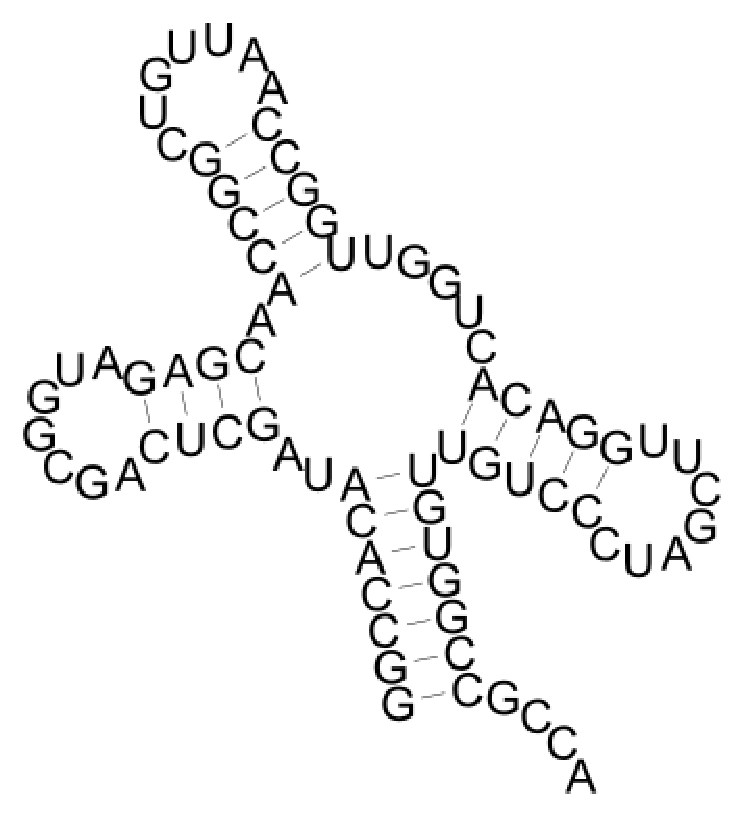
\includegraphics[width=\linewidth]{Figures/rna}
        \label{fig:rna}
        \caption{}
    \end{subfigure}
    \begin{subfigure}{.4\textwidth}
        \centering
        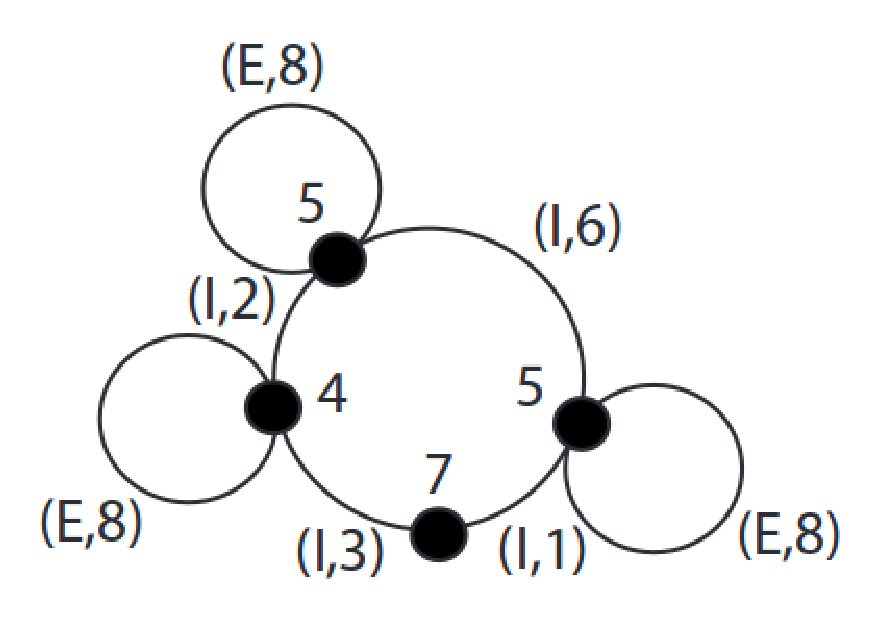
\includegraphics[width=\linewidth]{Figures/ldgrna}
        \label{fig:ldg}
        \caption{}
    \end{subfigure}
    \caption{a) RNA molecule graph representation and b) the same molecule represented
        as a labeled dual graph \cite{conf/psb/KarklinMH05}.}
    \label{fig:bio}
\end{figure}

Natural language processing is another field where graph representation is often used
as the basis for elaborate meaning extraction, as is the case for building opinion
lexicon from users review \cite{10.1371/journal.pone.0079294}, see Figure \ref{fig:wordrel}.

\begin{figure}[ht]
    \centering
    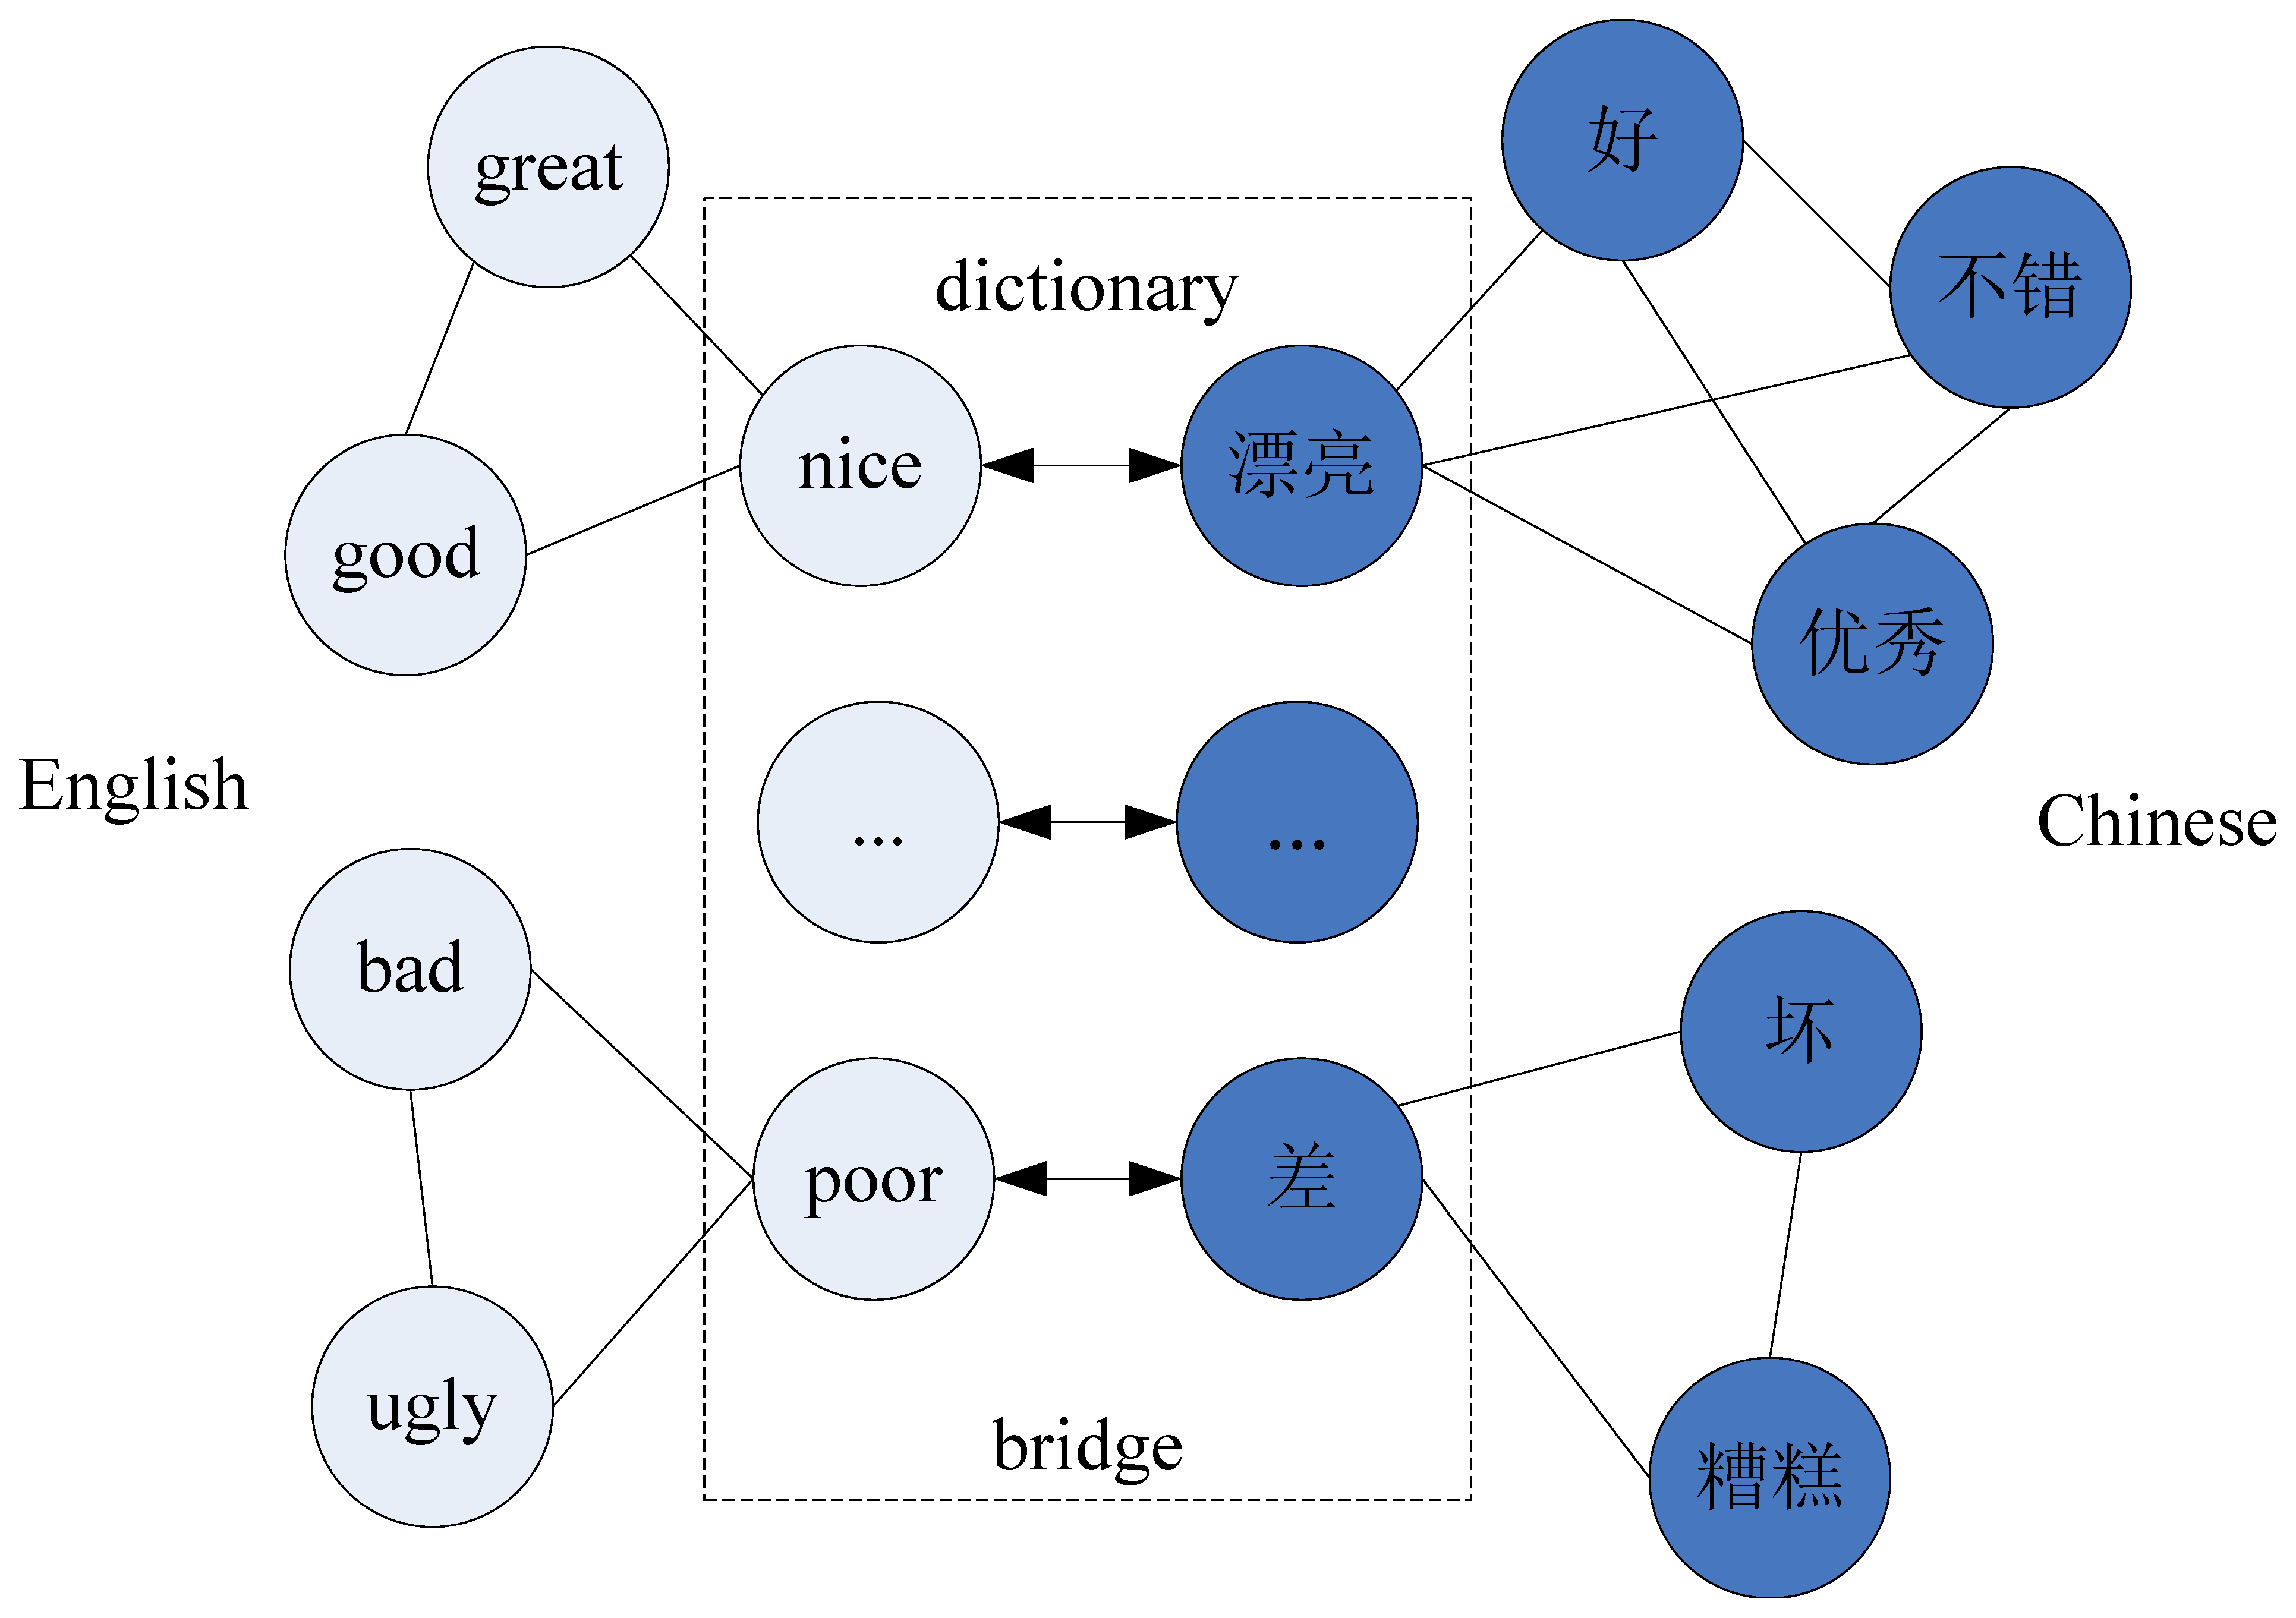
\includegraphics[width=.6\linewidth]{Figures/wordrel}
    \caption{Example of graph representation of words relationships in a multilingual
    context \cite{10.1371/journal.pone.0079294}.}
    \label{fig:wordrel}
\end{figure}

In computer vision a prominent application of the graph representation concerns
the so-called scene understanding or scene modelling task, where a scene is divided
into semantically meaningful areas which can be seen as nodes of a graph whose
edges are the adjacency relations between the areas \cite{journals/corr/abs-1108-4079},
an exemplification of which is given in Figure \ref{fig:scene}.

\begin{figure}[ht]
    \begin{subfigure}{.45\linewidth}
        \centering
        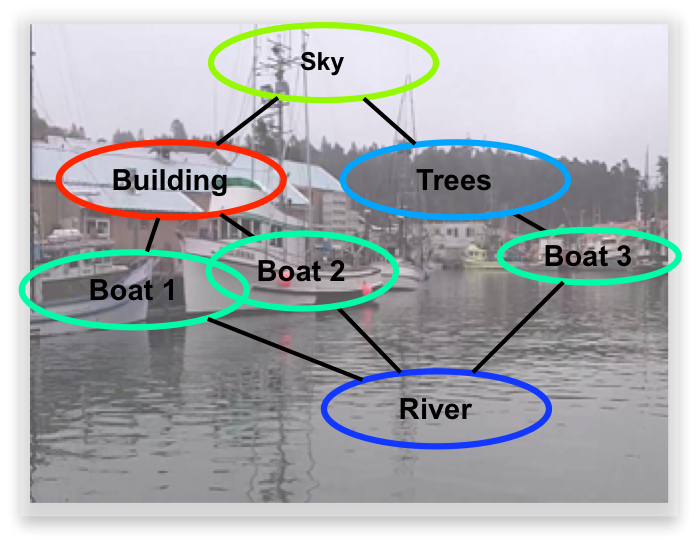
\includegraphics[width=\linewidth]{Figures/scene}
        \caption{}
        \label{fig:scene}
    \end{subfigure}
    \begin{subfigure}{.45\linewidth}
        \centering
        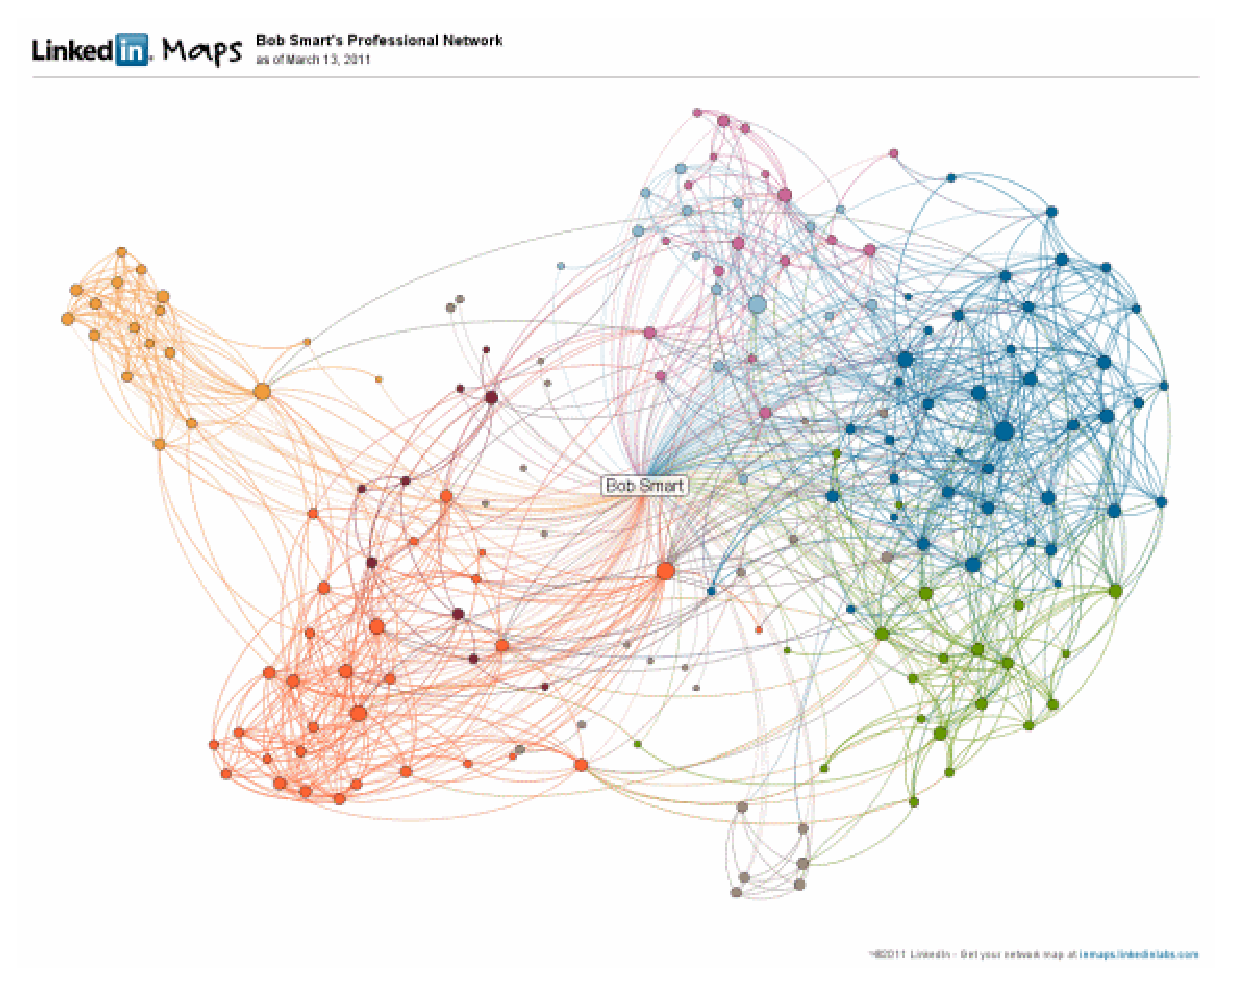
\includegraphics[width=\linewidth]{Figures/linkedin-social-maps}
        \caption{}
        \label{fig:network}
    \end{subfigure}
\caption{a) Scene understanding via graph decomposition in computer vision. b)
        LinkedIn's social maps show how a social network graph representation
        can quickly become very complex.}
\end{figure}

Finally  the graphs deriving from the inherently structured organization of every social
network can lead to a large number of mining possibilities given also the vast
amount of data available \cite{gundecha2012mining}.
Figure \ref{fig:network} gives an example of social network derived from a real-world
application.

%----------------------------------------------------------------------------------------

\section{Thesis contribution}

Given these premises, how can we learn from graphs? A first \emph{structure-based}
approach consist in designing an \emph{ad-hoc} vectorial representation for the
particular kind of graphs being considered.
This approach has one major downside which is that a renewed effort for the 
design of a new representation is needed every time a new type of data
is encountered.

Instead of focusing on the data, another approach is to adapt the existing methods
to work directly on graphs, thus permitting the exploitation of existing techniques.
Some recently proposed works \cite{DBLP:conf/sdm/MartinoNS12, NIPS2009_3813}
embed graph specific knowledge into well established \emph{kernel methods}
that, given the inherent decoupling between the data representation and the learning
algorithm that they provide (more on Section \ref{subsec:introkm}), make the
perfect fit for a more general approach.

\subsection{Kernel methods}
\label{subsec:introkm}

Kernel methods are a collection of techniques that rely on an implicit representation
of the data and a well defined measure of similarity between samples to perform
the learning task.
These methods have two main components: a domain specific function to compute the
samples pairwise similarity, called \emph{kernel function}, and a general purpose
learning algorithm, often called \emph{kernel machines}, to combine the information provided by the
kernel function in order to separate the samples.

Kernel functions are associated with a \emph{feature space} and define the similarity
score according to a set of features extracted from the samples.
Specific domain knowledge gets embedded in the learning process through the design of these
feature spaces and once the kernel function is defined, it becomes the only interface between the data
and the learning algorithm that never accesses its explicit representation.

Kernel machines are learning algorithms that employ the similarity measure defined
by kernel function to obtain sample separation in the implicit feature space and
map it back to the original input space from where the data was generated.
One of the most tried methods is the Support Vector Machine (SVM) \cite{Cortes&Vapnik:1995}
which is a binary classifier that tries to maximize the \emph{margin} between
two sets of labelled samples referring to their pairwise distance as their
similarity measure.

Graph kernel learning exploits this approach defining suitable kernel functions,
i.e. similarity measures, for graphs; a major challenge doing this is maintaining
an acceptable trade-off between expressiveness and efficiency.

\subsection{Hyper-parameter selection}
\label{sec:why}

Most learning methods have parameters that need tuning, i.e. in order to achieve
good generalization performances each value has to be selected from a set of
possible choices according to a performance measure.

The selection procedure often involves a limited search on the parameter space
that is, a set of values for each parameter is fixed and all the combinations
are tested to find the best one.
However, in order to be useful the sampling on the parameter space needs to be adequate:
the complexity of this search can still be daunting because it depends from the
number of parameters and the cardinality of each values set.

In the context of kernel learning hyper-parameters can be found on two levels:
parameters relative to the kernel function and parameters that belongs to the
kernel machine (solver).
The parameters of the former typically influence the feature space being generated,
directly affecting the expressiveness of the similarity measure, i.e. the ability
to discern between different samples.
The parameters of the solver are usually employed as regularization factors,
as is the case for SVMs, where it is used to balance the trade-off between a good
(generalizing) separator and empirical error.
Once the solver has been chosen, the parameter space is determined by the kernel
hyper-parameters hence, the kernel choice can greatly affect the computational
performances of the whole approach.
Moreover, often the kernel selection has to be validated too, thus increasing the
computational burden even more.

\subsection{Proposed solution}

To address this last point a different approach, called \emph{multiple kernel learning} (MKL),
has been developed which allows to combine different kernel functions into a single learning process.
From the plethora of implementations available in literature \cite{journals/jmlr/GonenA11},
we selected EasyMKL, a recently proposed state-of-the-art MKL implementation
\cite{aiolli2015easymkl} with a linear complexity bound w.r.t. the input size.
This algorithm effectively finds the best possible linear combination of the
input kernels as a weighed sum.

Furthermore, graph kernels typically become more computationally expensive the
more expressive they get.
Combining a number of more efficient although less expressive kernels could
lead to a boost in performance due to the inherent enrichment of the feature set
while maintaining acceptable performances.

We here propose a methodology to avoid the cumbersome process of kernel
hyper-parameter selection, employing at once all the kernels that would have been calculated
according to the parameter space search (e.g. grid search, see Section \ref{subsubsec:grid})
with EasyMKL.
We discuss also how a process of kernel orthogonalization can improve the algorithm space
consumption while boosting the performances.

With this approach the whole process of hyper-parameter selection has been streamlined and
lifted from the kernels to the learning machine, effectively eliminating the need to test each
kernel in isolation.

%----------------------------------------------------------------------------------------

\section{Thesis outline}
This document is organized as follows: in Chapter \ref{Chapter2} we delve into
the background details that are necessary to fully understand the proposed idea;
we cover the basics of machine learning and kernel methods and see some examples
of kernel combination techniques.
The main ideas behind this work are exposed in Chapter \ref{Chapter3} where we
discuss in detail our approach, the conceptual steps involved and the solutions
to the problems encountered.
Chapter \ref{Chapter4} covers the experimental part of the thesis, where we present
our results and finally in Chapter \ref{Chapter5} we draw conclusions and explain
how some ideas proposed here can be further explored.

%----------------------------------------------------------------------------------------

% vim: spell spelllang=en_gb
